\section{Performance}

\begin{frame}
	\frametitle{Strong Scaling}
	\begin{figure}
		\centering
		\makebox[\textwidth]{%
		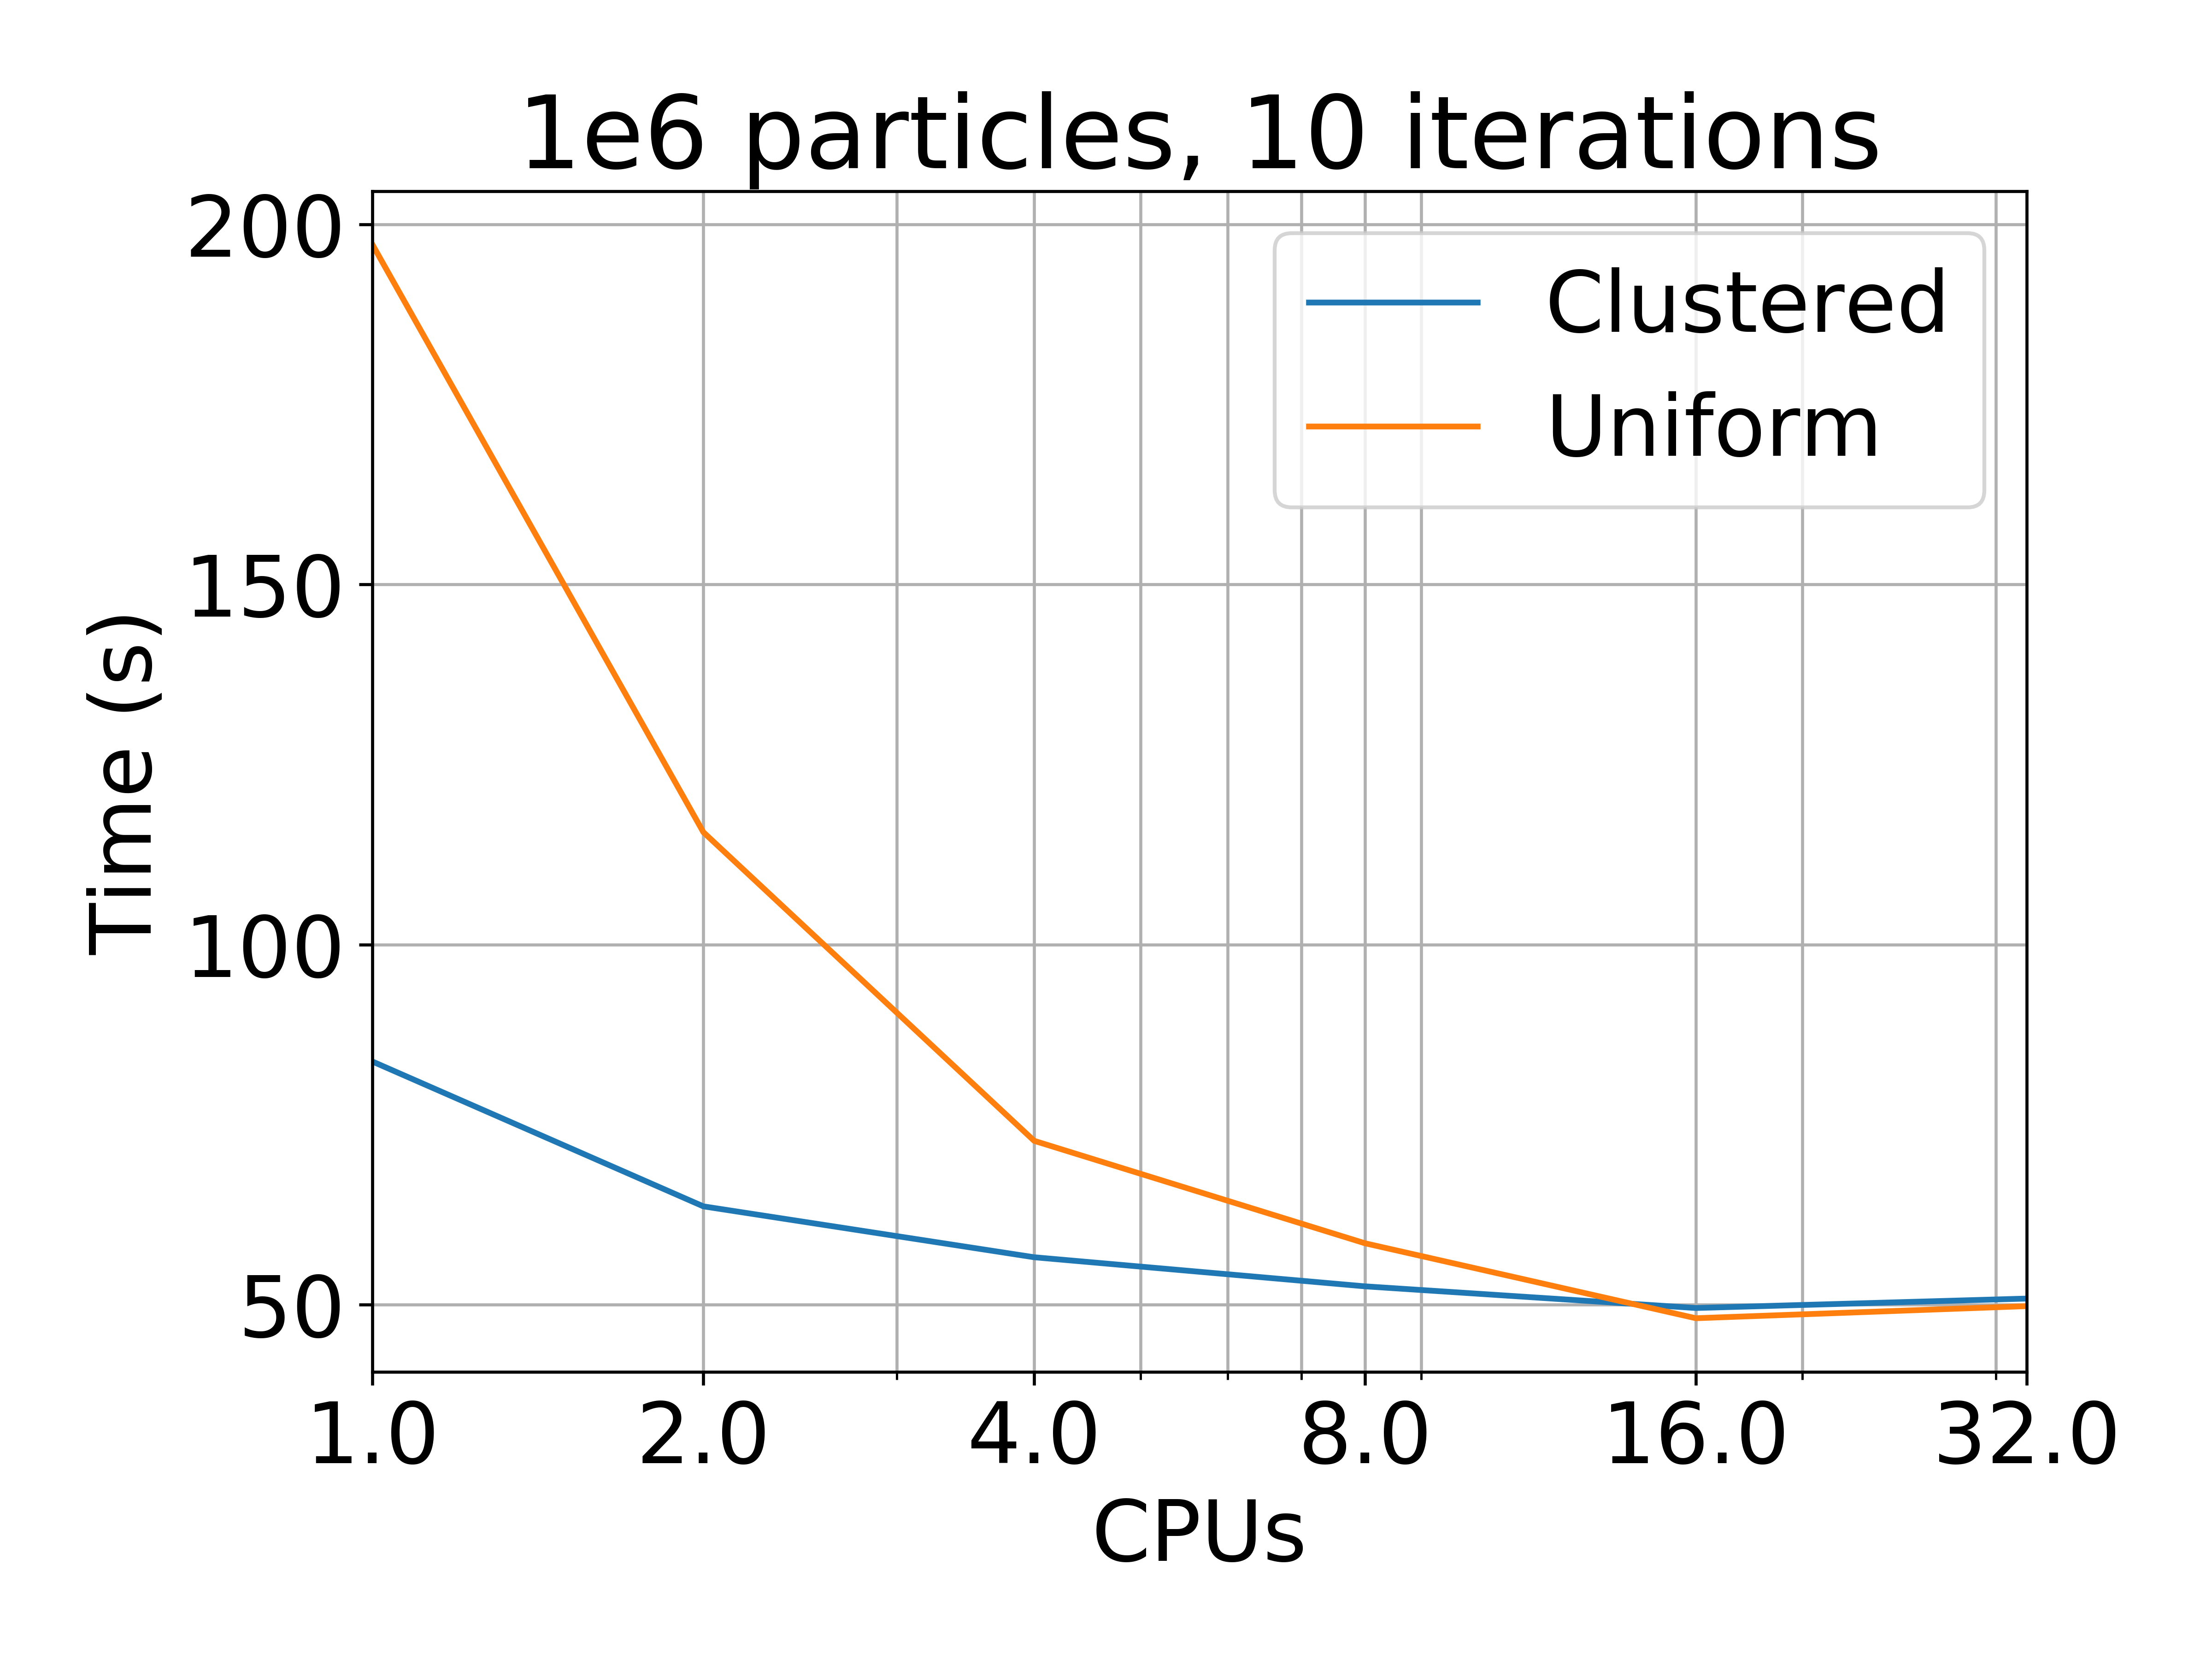
\includegraphics[width=0.49\paperwidth]{inclfigs/strong_time.png}
		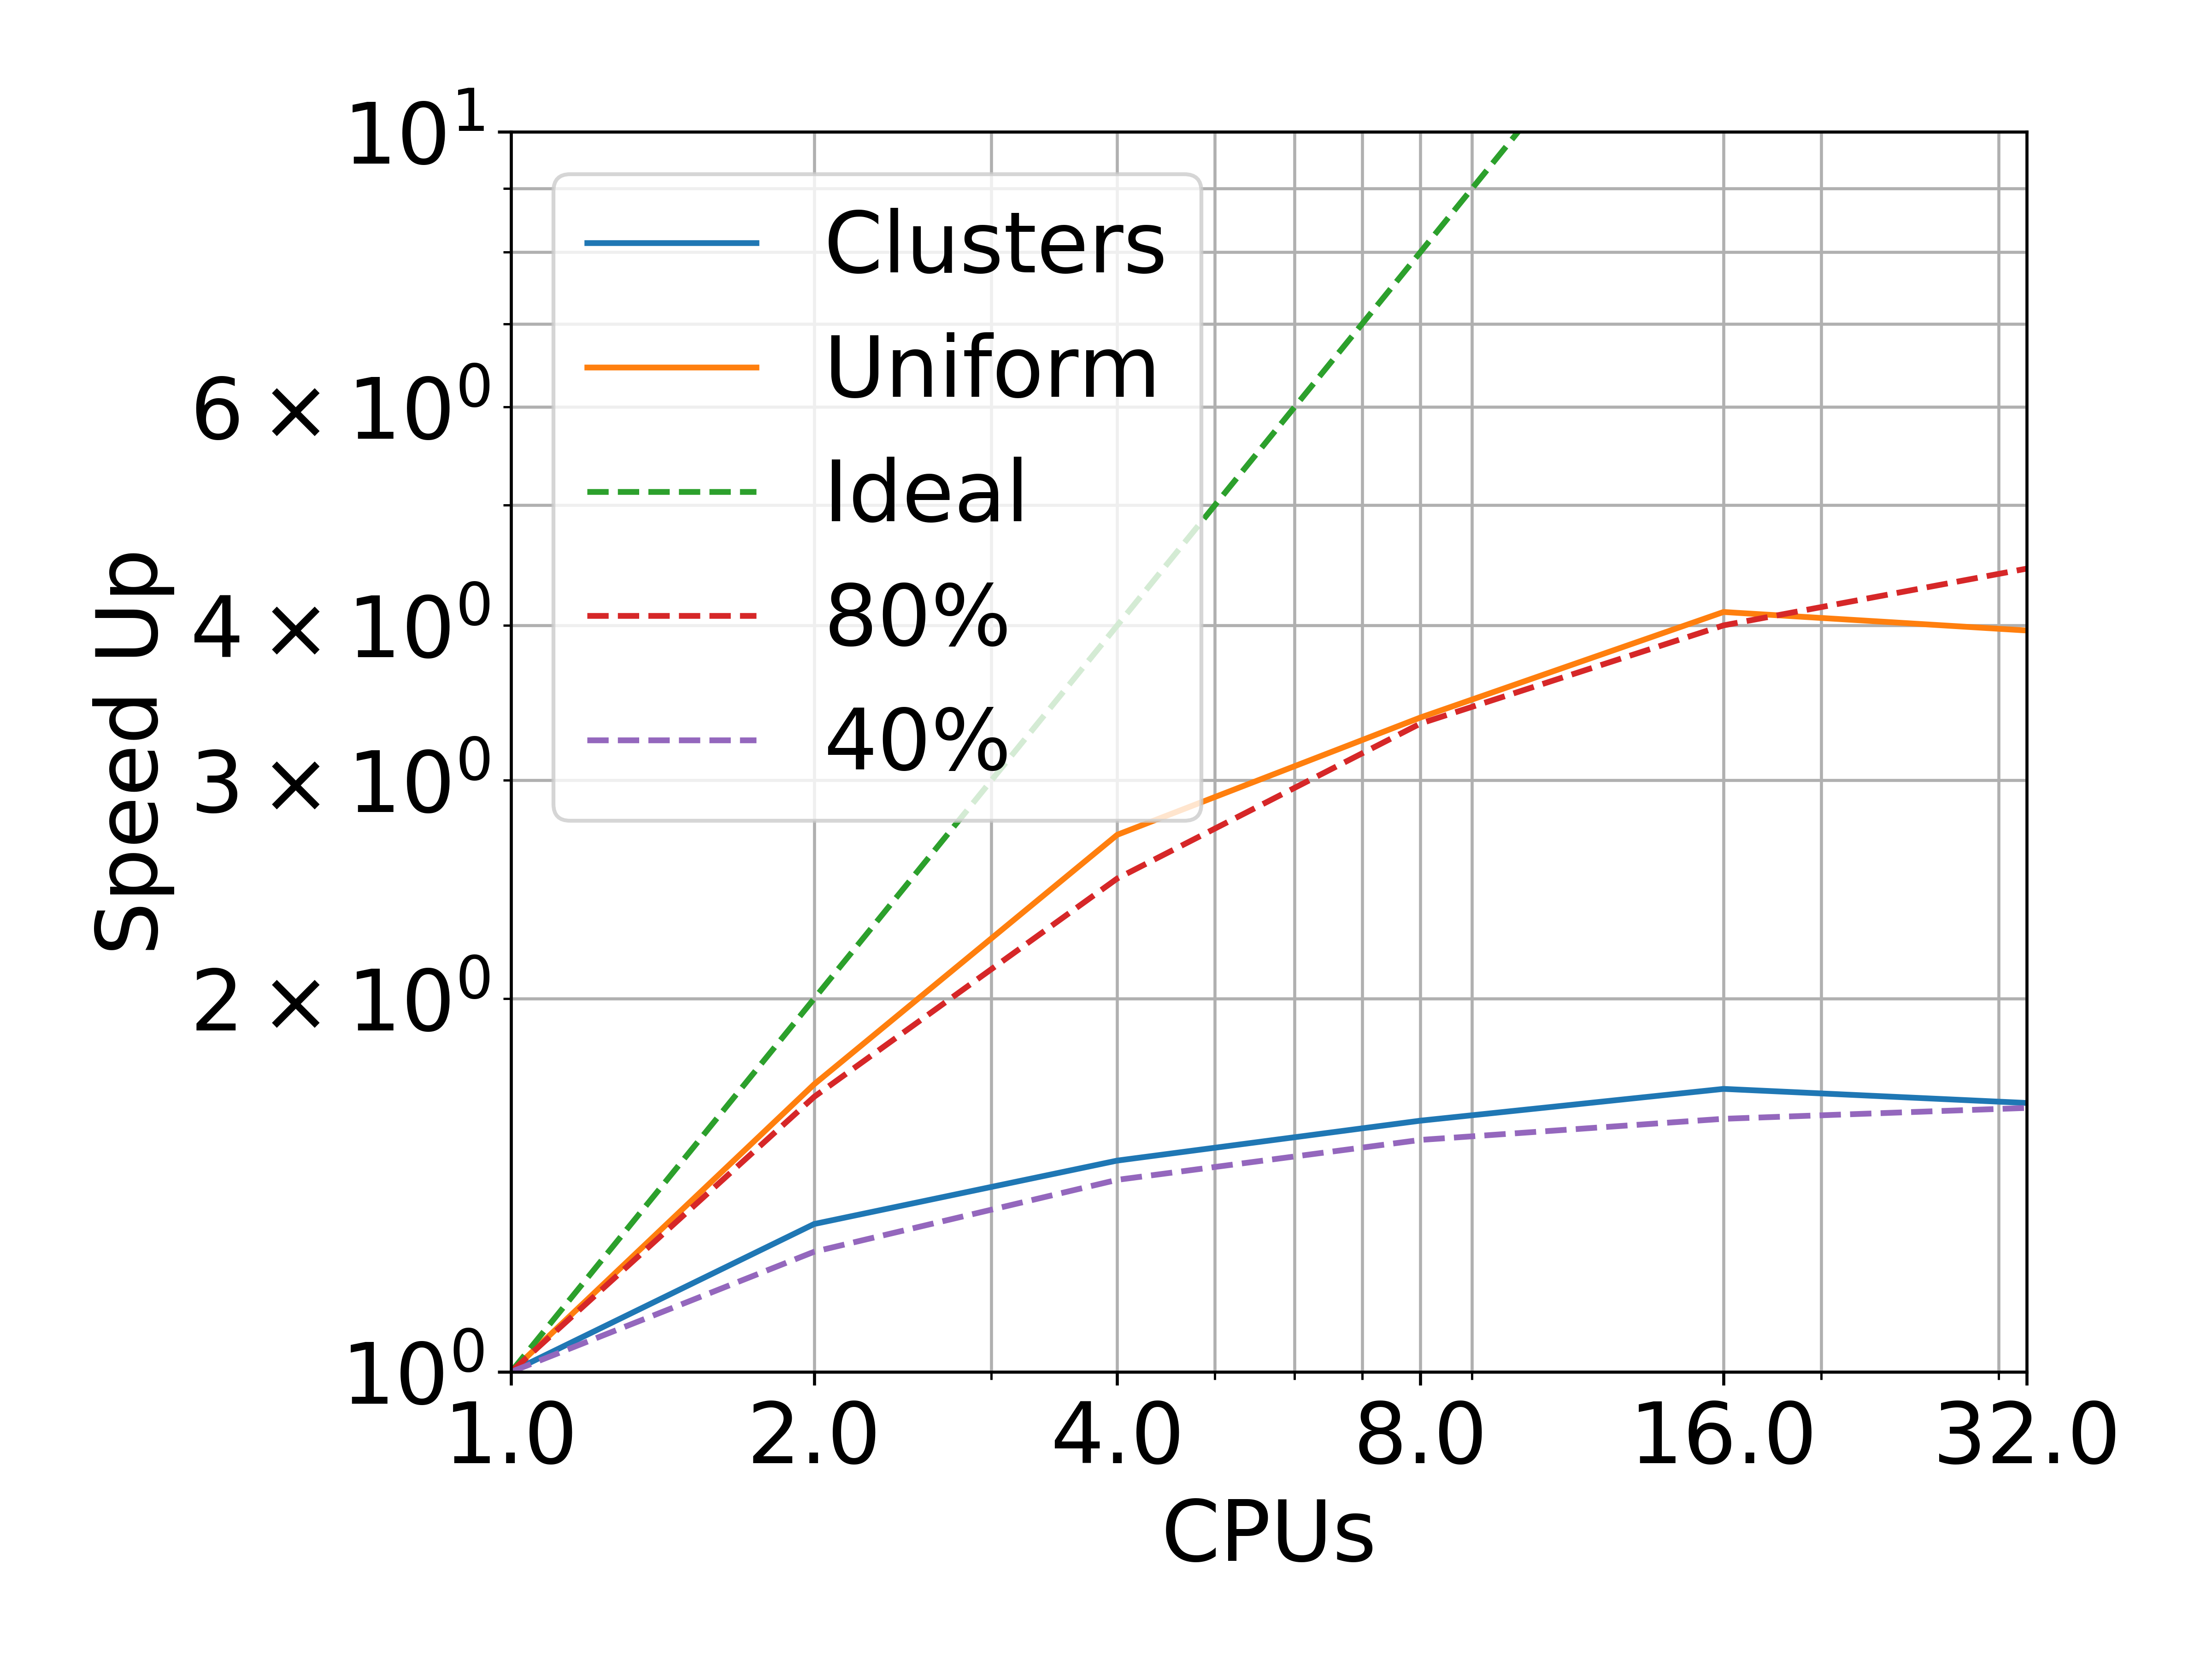
\includegraphics[width=0.49\paperwidth]{inclfigs/strong_speedup.png}
		}
	\end{figure}
\end{frame}

\begin{frame}
	\frametitle{Weak Scaling}
	\begin{figure}
		\centering
		\makebox[\textwidth]{%
		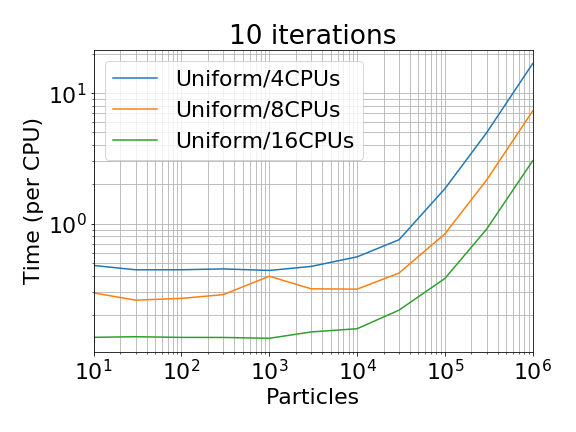
\includegraphics[width=0.49\paperwidth]{inclfigs/weak_time.png}
		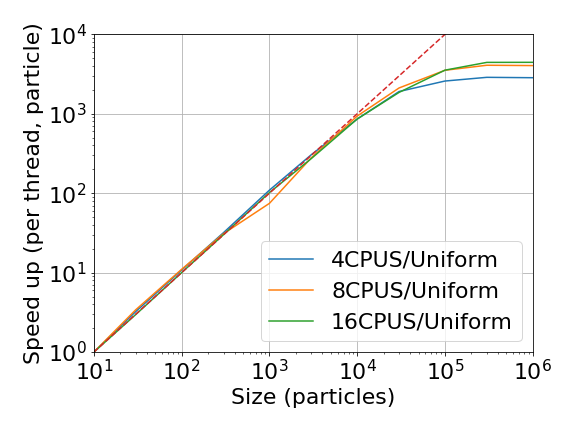
\includegraphics[width=0.49\paperwidth]{inclfigs/weak_speedup.png}
		}
	\end{figure}
\end{frame}

\begin{frame}
	\frametitle{Hotspots}
	\begin{figure}
		\centering
		\makebox[\textwidth]{%
		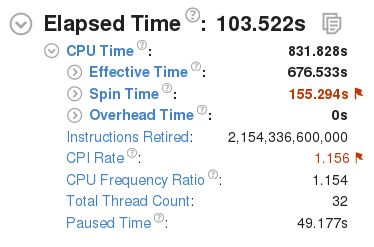
\includegraphics[width=0.49\paperwidth]{inclfigs/par-spintime.png}
		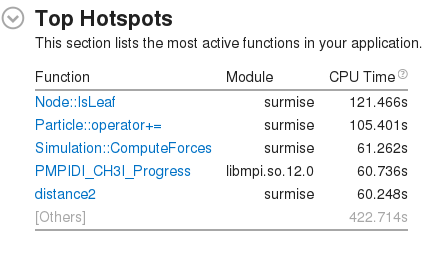
\includegraphics[width=0.49\paperwidth]{inclfigs/par-hotspots.png}
		}
	\end{figure}
\end{frame}

\begin{frame}
\frametitle{Bottom-Up}
	\begin{figure}
		\centering
		\onslide<1-3>{\makebox[\textwidth]{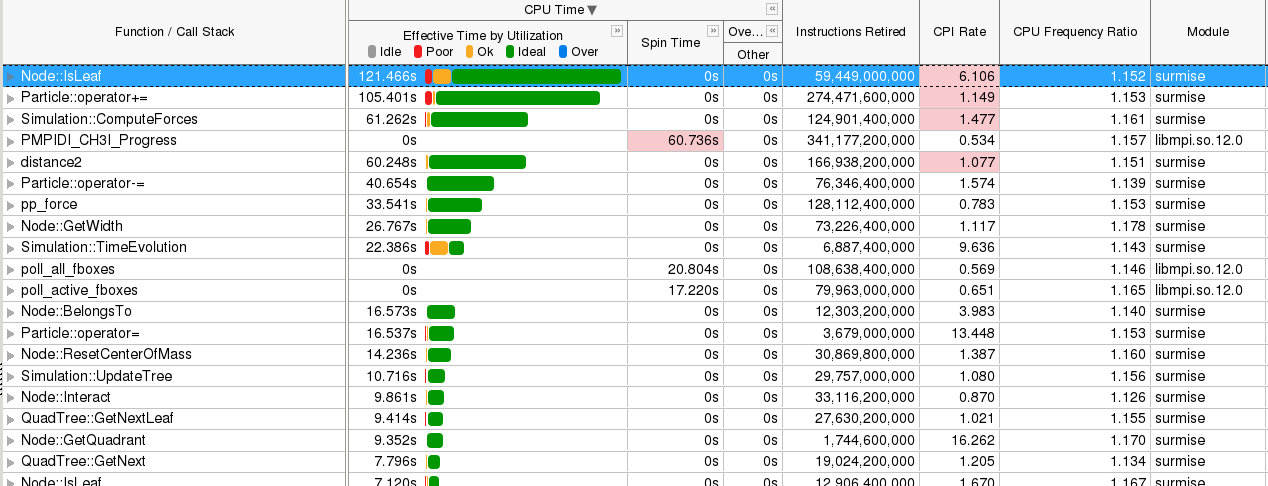
\includegraphics[width=\paperwidth]{inclfigs/par-bottomup.png}}}\\[10pt]
		\onslide<2-3>{%
		\only<2>{\makebox[\textwidth]{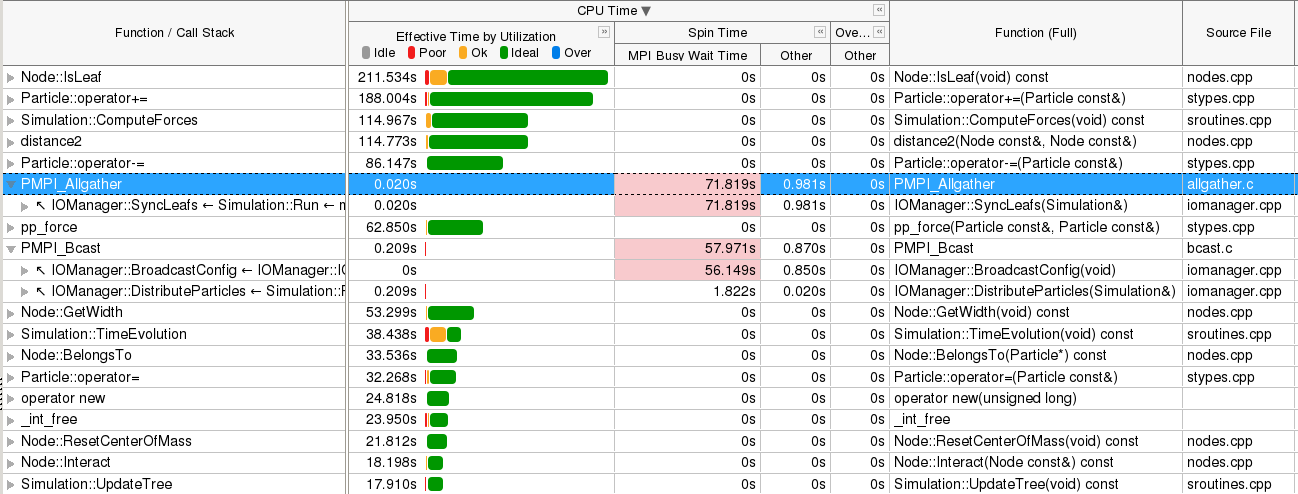
\includegraphics[width=\paperwidth,trim={0 1.5cm 0 1.5cm},clip]{inclfigs/par-mpi.png}}}
		\onslide<3>{\makebox[\textwidth]{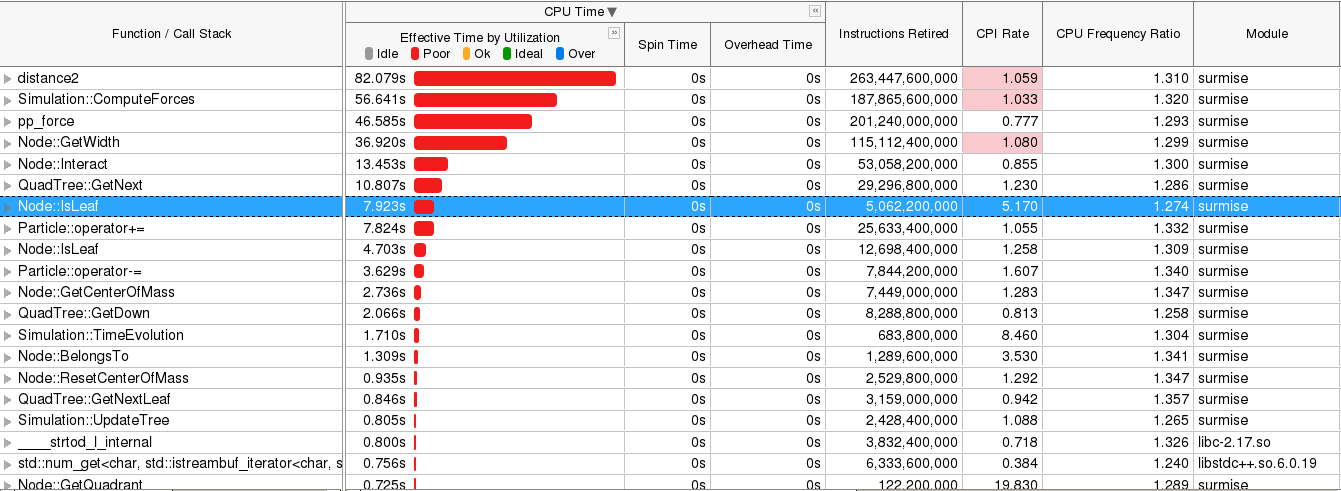
\includegraphics[width=\paperwidth,trim={0 1.72cm 0 1cm},clip]{inclfigs/seq-bottomup.png}}}
		}
	\end{figure}
\end{frame}

\begin{frame}
\frametitle{CPU Time}
	\begin{figure}
		\centering
		\makebox[\textwidth]{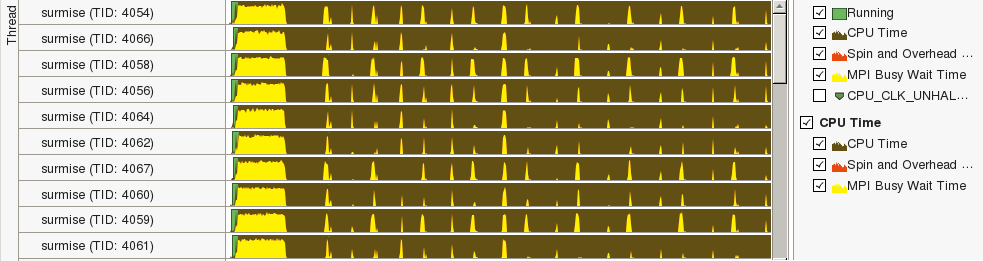
\includegraphics[width=\paperwidth]{inclfigs/par-heatmap.png}}
	\end{figure}
\end{frame}